% Options for packages loaded elsewhere
\PassOptionsToPackage{unicode}{hyperref}
\PassOptionsToPackage{hyphens}{url}
\PassOptionsToPackage{dvipsnames,svgnames,x11names}{xcolor}
\documentclass[
]{ltjsarticle}
\usepackage{xcolor}
\usepackage[margin=22mm]{geometry}
\usepackage{amsmath,amssymb}
\setcounter{secnumdepth}{-\maxdimen} % remove section numbering
\usepackage{iftex}
\ifPDFTeX
  \usepackage[T1]{fontenc}
  \usepackage[utf8]{inputenc}
  \usepackage{textcomp} % provide euro and other symbols
\else % if luatex or xetex
  \usepackage{unicode-math} % this also loads fontspec
  \defaultfontfeatures{Scale=MatchLowercase}
  \defaultfontfeatures[\rmfamily]{Ligatures=TeX,Scale=1}
\fi
\usepackage{lmodern}
\ifPDFTeX\else
  % xetex/luatex font selection
\fi
% Use upquote if available, for straight quotes in verbatim environments
\IfFileExists{upquote.sty}{\usepackage{upquote}}{}
\IfFileExists{microtype.sty}{% use microtype if available
  \usepackage[]{microtype}
  \UseMicrotypeSet[protrusion]{basicmath} % disable protrusion for tt fonts
}{}
\makeatletter
\@ifundefined{KOMAClassName}{% if non-KOMA class
  \IfFileExists{parskip.sty}{%
    \usepackage{parskip}
  }{% else
    \setlength{\parindent}{0pt}
    \setlength{\parskip}{6pt plus 2pt minus 1pt}}
}{% if KOMA class
  \KOMAoptions{parskip=half}}
\makeatother
\usepackage{longtable,booktabs,array}
\newcounter{none} % for unnumbered tables
\usepackage{calc} % for calculating minipage widths
% Correct order of tables after \paragraph or \subparagraph
\usepackage{etoolbox}
\makeatletter
\patchcmd\longtable{\par}{\if@noskipsec\mbox{}\fi\par}{}{}
\makeatother
% Allow footnotes in longtable head/foot
\IfFileExists{footnotehyper.sty}{\usepackage{footnotehyper}}{\usepackage{footnote}}
\makesavenoteenv{longtable}
\usepackage{graphicx}
\makeatletter
\newsavebox\pandoc@box
\newcommand*\pandocbounded[1]{% scales image to fit in text height/width
  \sbox\pandoc@box{#1}%
  \Gscale@div\@tempa{\textheight}{\dimexpr\ht\pandoc@box+\dp\pandoc@box\relax}%
  \Gscale@div\@tempb{\linewidth}{\wd\pandoc@box}%
  \ifdim\@tempb\p@<\@tempa\p@\let\@tempa\@tempb\fi% select the smaller of both
  \ifdim\@tempa\p@<\p@\scalebox{\@tempa}{\usebox\pandoc@box}%
  \else\usebox{\pandoc@box}%
  \fi%
}
% Set default figure placement to htbp
\def\fps@figure{htbp}
\makeatother
\setlength{\emergencystretch}{3em} % prevent overfull lines
\providecommand{\tightlist}{%
  \setlength{\itemsep}{0pt}\setlength{\parskip}{0pt}}
\usepackage{bookmark}
\IfFileExists{xurl.sty}{\usepackage{xurl}}{} % add URL line breaks if available
\urlstyle{same}
\hypersetup{
  colorlinks=true,
  linkcolor={Maroon},
  filecolor={Maroon},
  citecolor={Blue},
  urlcolor={Blue},
  pdfcreator={LaTeX via pandoc}}

\author{}
\date{}

\begin{document}

\section{論文13:位置は読まれていなかった ---
符号セクター・双対性定理・読み出し階層・導出時計}\label{ux8ad6ux658713ux4f4dux7f6eux306fux8aadux307eux308cux3066ux3044ux306aux304bux3063ux305f-ux7b26ux53f7ux30bbux30afux30bfux30fcux53ccux5bfeux6027ux5b9aux7406ux8aadux307fux51faux3057ux968eux5c64ux5c0eux51faux6642ux8a08}

\textbf{著者}: 木原範昭 \textbf{作成}: 2026年6月12日 \textbf{版}:
v1.0(確定版。v0.2=第1回査読{[}中改訂{]}反映、v1.0=第2回査読{[}採録・軽微修正条件付き{]}の
R1〜R5 を反映) \textbf{DOI(本版)}: 10.5281/zenodo.20665634 /
\textbf{Concept DOI}: 10.5281/zenodo.20665633 \textbf{ライセンス}: CC BY
4.0 \textbf{シリーズ}: 波長空間と周波数空間の双対幾何(論文1〜12
の続編、第13篇)

\begin{center}\rule{0.5\linewidth}{0.5pt}\end{center}

\subsection{要旨}\label{ux8981ux65e8}

「離散状態は位置と時間に往復写像できるのか」---
本シリーズの体系(3公理:νλ=1・零点½・非対称1ビット+配置読み・記録原理)に対する最古の問いに、公理在庫の\textbf{追加ゼロ}で答える。主結果:(1)
\textbf{位置は新しい自由度ではなく、辞書の未読部分だった}。離散位置=波の符号セクター(¼周期オフセット:cos→sin→−cos→−sin)であり、これは論文5
の辞書が最初から持っていたデータの読み出し方の変更にすぎない ---
状態空間への追加は厳密にゼロ(定理1)。(2)
\textbf{空間は導出される}:位置空間=保存量格子(電荷様) \(\mathbb{Z}^4\)
の Pontryagin 双対
\(T^4\)(指標群)であり、並進・回転・反転の三対称性は仮定ではなく\textbf{双対性の定理}である(定理2)。背景時空の実体は仮定されない
--- 位置空間は関係データ(線係数)のチャートである。(3)
\textbf{読み出しは三層}:強度縞のスカラーデータ(縞間隔)は関係クラスを11種までしか分離しないが、線位置データは13種、\textbf{枝チャネル(複素線係数)は全21軌道を完全分離}する(定理3、全数計数
11⊂13⊂21)---
「位置は読まれていなかった」の定量的実証であり、強度のみの読みでは原理的に失われる情報の所在を確定する。(4)
\textbf{¼単位変位定理}:断片の¼格子変位は枝チャネルの位相クラス(Z₄)として厳密に読める(定理4)---
連続位置はこの¼桁の階層完備化である(写像の構成は論文15、同時期公開予定)。(5)
\textbf{時間は解決される --- ただし位置とは非対称に}:時計周波数
\(\nu_t=\sqrt{s}\) の標的 \(\nu_t^2\) は\textbf{全ての奇数}を間隔2で走る
---
これは\textbf{ガウスの三角数定理による範囲無制限の証明付き定理}である(定理5:奇数
\(s\) に対し \((s-1)/2\)
は4つの三角数の和であり、ガウスの定理{[}全自然数は3つの三角数の和{]}により常に解がある)。可能な限り最も規則的なスペクトルが、証明済みの主張として立つ。正写像は4軸とも厳密である一方、\textbf{t
には独立な逆写像が存在しない}(定理6):\(\nu_t\)
は空間配置のノルムとして導出されるため、t
は丸めるべき独立の目盛りを持たない。これは欠陥ではなく「t
は基本自由度でない ---
観測の結果選ばれたように見えるだけ」という全軸対称の原則の定理形である。t
は xyz
より\textbf{易しい}。本論文は標準理論の再導出を主張しない。物理的同一視は行わない。

\begin{center}\rule{0.5\linewidth}{0.5pt}\end{center}

\subsection{1. 序論}\label{ux5e8fux8ad6}

\subsubsection{1.1
五十年の問い}\label{ux4e94ux5341ux5e74ux306eux554fux3044}

連続な位置 \(x\) と時間 \(t\)
は、離散の状態記述とどう両立するのか。この問いは本シリーズの体系に対して次の形を取る:

\begin{quote}
体系の状態データ(占有セル・枝・帳簿)から、位置と時間は\textbf{読み出せる}のか。読み出せるなら、それは状態空間への追加(新しい自由度)を要するのか。
\end{quote}

本論文の答え:\textbf{読み出せる。追加はゼロ}。位置は辞書(論文5)が最初から持っていた符号セクターの読み替えであり、時間は保存ノルムの導出量である。必要だったのは公理でも拡張でもなく、\textbf{読み出し原理の変更}だった
--- ゆえに本論文の表題は「位置は読まれていなかった」である。

\subsubsection{1.2
主張しないこと}\label{ux4e3bux5f35ux3057ux306aux3044ux3053ux3068}

\begin{enumerate}
\def\labelenumi{(\roman{enumi})}
\tightlist
\item
  連続座標への明示的な写像の構成(混合基数展開・読み出し演算・逆写像)は論文15
  が行う ---
  本論文はその\textbf{定理的基礎}(何が読めるか・何が導出量か)である。(ii)
  時間方向の選択(どの軸が t に見えるか)と振幅の地位は論文14。(iii)
  \textbf{本論文は経路振幅の集計規則(測度)を選定しない}(進行中の測度線=論文16
  の管轄、同時期公開予定)。(iv) 物理的同一視は行わない。
\end{enumerate}

\subsection{2.
前提(最小限の再掲)}\label{ux524dux63d0ux6700ux5c0fux9650ux306eux518dux63b2}

論文5 の辞書:セル \(k\in\mathbb{Z}^4\) ↔ 積波
\(\Phi_k=\prod_j\varphi_{k_j}(x_j)\)、枝は
\(k_j>0\)=cos・\(k_j<0\)=sin。配置読み(論文7):状態=占有セルの集合=波そのもの。記録(論文6/12):ホログラム
\(I=\Psi^2\)、物理的内容は線係数(関係データ)。帳簿:\(s=\sum_j(|k_j|+\tfrac12)^2\)、\(\varepsilon=(-1)^{\Sigma|k_j|}\)。

\textbf{固定するゲージデータ(全列挙)}: マーキング
\(u\)(時間読み軸)・軸ごとの向き付け
\(Z_2^{4}\)(枝の正方向)・基準断片(原点)。定理1・4 の符号セクター/Z₄
読みは\textbf{これらに相対的なゲージ相対量}である(§6 限界1
の「相対量」はこの列挙に接続する)。

\textbf{内部用語宣言}:
本論文の「位置」「時間」は体系内の読み出し量の名であり、物理量との同一視を含意しない(命名規律:保存量は「電荷様」等の警報つき表記)。

\subsection{3. 位置の解決}\label{ux4f4dux7f6eux306eux89e3ux6c7a}

\subsubsection{3.1
定理1(符号セクター=離散位置、状態追加ゼロ)}\label{ux5b9aux74061ux7b26ux53f7ux30bbux30afux30bfux30fcux96e2ux6563ux4f4dux7f6eux72b6ux614bux8ffdux52a0ux30bcux30ed}

\begin{quote}
\textbf{定理1}: 基本波の¼周期並進 \(T_{1/4}\)
は辞書の枝・符号を巡回する:\(\cos\to\sin\to-\cos\to-\sin\)(\(d\to d+1\bmod 4\))。したがって\textbf{辞書の(枝,
符号)の組=¼周期オフセット=離散位置}であり、位置の導入に新しい状態は一つも要らない。
\end{quote}

\textbf{証明}(2行):\(\cos(\theta-\pi/2)=\sin\theta\)、\(\sin(\theta-\pi/2)=-\cos\theta\)
--- ¼並進は三角恒等式の巡回そのもの。∎ 機械確認(②):全数
4/4(図1a)。これまで「同じ状態の別表現」と扱われてきた符号セクターが、実は位置データだった
--- 読み出し原理の変更だけが必要だった。

\subsubsection{3.2
空間=保存量格子の双対(定義・一般定理・整合定理の三分割)}\label{ux7a7aux9593ux4fddux5b58ux91cfux683cux5b50ux306eux53ccux5bfeux5b9aux7fa9ux4e00ux822cux5b9aux7406ux6574ux5408ux5b9aux7406ux306eux4e09ux5206ux5272}

\textbf{定義2}: 位置空間を、保存量格子(電荷様)\(\mathbb{Z}^4\)
の指標群(Pontryagin 双対)\(T^4=\mathrm{Hom}(\mathbb{Z}^4,U(1))\)
として\textbf{定める}(双対チャート)。

\begin{quote}
\textbf{定理2a(一般論 --- 証明事項であり検証対象ではない)}:
この定義の下で (i) 並進対称性=指標群の群構造、(ii)
回転(B₄)対称性=格子自己同型の双対作用、(iii)
反転対称性=複素共役、はいずれも Pontryagin 双対性の標準的な定理である。
\end{quote}

\begin{quote}
\textbf{定理2b(モデル固有の整合)}: 記録の物理的内容(線係数)は
\(\mathbb{Z}^4\) 上の関数であり、定理1 の符号セクター読みは各軸の
\(Z_4\subset U(1)\)
としてこの双対チャートに埋め込まれる(¼並進=指標の¼回転)。機械確認(②):定理1
の 4/4 巡回がそのまま \(Z_4\hookrightarrow U(1)\) の整合確認である。
\end{quote}

帰結(背景独立性):位置空間は実体として仮定される容れ物ではなく、関係データ(線係数=格子で添字づけられた量)の双対チャートである。連続位置は¼桁の階層完備化として得られる(図1b;明示的構成は論文15
定理2、同時期公開予定)。

\subsubsection{3.3 定理3(読み出し階層
11⊂13⊂21)}\label{ux5b9aux74063ux8aadux307fux51faux3057ux968eux5c64-111321}

shell-9 の全64セルの対(2016対)の関係クラス(B₄×入替軌道)は
\textbf{21}。読み出し層ごとの分離能(全数計数、図2):

{\def\LTcaptype{none} % do not increment counter
\begin{longtable}[]{@{}
  >{\raggedright\arraybackslash}p{(\linewidth - 4\tabcolsep) * \real{0.3333}}
  >{\raggedright\arraybackslash}p{(\linewidth - 4\tabcolsep) * \real{0.3333}}
  >{\raggedright\arraybackslash}p{(\linewidth - 4\tabcolsep) * \real{0.3333}}@{}}
\toprule\noalign{}
\begin{minipage}[b]{\linewidth}\raggedright
読み出し層
\end{minipage} & \begin{minipage}[b]{\linewidth}\raggedright
可読データ
\end{minipage} & \begin{minipage}[b]{\linewidth}\raggedright
分離クラス数
\end{minipage} \\
\midrule\noalign{}
\endhead
\bottomrule\noalign{}
\endlastfoot
スカラー縞 & 縞間隔 \((|\Delta|^2,|\Sigma|^2)\) 無順序 &
\textbf{11}(順序つきでも18) \\
線位置縞 & 非符号線対 \(\{[u{+}v],[u{-}v]\}\) & \textbf{13} \\
枝チャネル & 複素線係数(cos/sin 分解) & \textbf{21 = 完全分離} \\
\end{longtable}
}

\begin{quote}
強度のみの読み(従来の縞)は、21軌道のうち\textbf{スカラー縞で10クラス分(21→11;併合の対構造は未確認)、線位置縞で8対(全て対であることを検証済み)}の区別を原理的に失う。\textbf{全情報を回収する読みは枝チャネルのみ}
---
「位置は読まれていなかった」の定量形。線位置縞で併合される8対の軌道は全て「和線と差線の取り違え=相対符号の不可読」型である。
\end{quote}

\subsubsection{3.4 定理4(¼単位変位の可読性 ---
成分依存則)}\label{ux5b9aux74064uxbcux5358ux4f4dux5909ux4f4dux306eux53efux8aadux6027-ux6210ux5206ux4f9dux5b58ux5247}

\begin{quote}
\textbf{定理4}: 断片の¼格子変位は、周波数成分 \(m\)
の線の位相クラス(Z₄)を \textbf{\(m\bmod 4\)
シフト}する(一般則)。基本成分(\(m=1\))では +1
であり、奇数成分(\(m\bmod4\in\{1,3\}\))では可逆ゆえ変位は読める。
\end{quote}

「+1」は基本成分に限る(多成分断片では成分ごとに \(m\bmod4\);指摘 \#3
による精密化)。論文15 の桁規約(\(d^{(0)}\)、\(\min(c,k{-}1)\)
クリップ)とはこの一般則の \(m=1\)
截面で整合する。機械確認(③標本):縞シフトテスト2件(三脚¼回転・環反転)PASS
---
標本検査であり全数ではない。これが離散位置の操作的読み出しであり、階層への拡張(ピーリング復号)と連続化は論文15
§5(同時期公開予定)。

\subsection{4. 時間の解決}\label{ux6642ux9593ux306eux89e3ux6c7a}

\subsubsection{4.1 定理5(時計の標的=全奇数 ---
証明付き)}\label{ux5b9aux74065ux6642ux8a08ux306eux6a19ux7684ux5168ux5947ux6570-ux8a3cux660eux4ed8ux304d}

\begin{quote}
\textbf{定理5}: 時計周波数の二乗 \(\nu_t^2=s=\sum_j(|k_j|+\tfrac12)^2\)
の値域は\textbf{ちょうど全ての奇数}である(間隔2)。
\end{quote}

\textbf{証明}: (値域⊆奇数)\(s=\sum_j|k_j|(|k_j|+1)+1\) で、各
\(|k_j|(|k_j|+1)\) は連続整数の積ゆえ\textbf{偶} --- よって \(s\)
は常に奇数。(奇数⊆値域)任意の奇数 \(s\) に対し
\((s-1)/2=\sum_j|k_j|(|k_j|+1)/2=\sum_j T_{|k_j|}\)
は\textbf{4つの三角数の和}への分解問題であり、ガウスの三角数定理(全自然数は3つの三角数の和;1796年の
Eureka)により常に解がある(\(T_0=0\)
を加えて4つにする)。∎(証明の同定:第1回査読 \#1、claude.ai)

機械確認(②):奇数199以下で100/100到達(図3a)。時間の目盛りは「飛び飛びで不規則」ではなく、可能な限り最も規則的である
--- \textbf{証明済みの主張として}。各 \(s\) での刻みは
\(\Delta t=1/\sqrt{s}\)(図3b)--- 論文8 の内部時間 \(t=\sum 1/\sqrt{s}\)
と同一の構成。

\subsubsection{4.2 定理6(t
に独立な逆写像はない)}\label{ux5b9aux74066t-ux306bux72ecux7acbux306aux9006ux5199ux50cfux306fux306aux3044}

\begin{quote}
\textbf{定理6(t の因子化)}:
正写像(状態→4軸の読み)は4軸とも厳密に存在する。逆向きについて:\textbf{記録から読める任意の
t 値は \(s\) の関数を経由して因子化する} --- すなわち、t に \(s\)
と独立な分解能を与える読み出しは存在しない。xyz
の各軸が持つ独立の丸め(逆写像、論文15 D4)に対応する操作が、t
には\textbf{ない}。
\end{quote}

\textbf{証明スケッチ(在庫監査)}:
状態データの台帳は占有セル(4軸の整数)・枝・符号で尽きる(配置読み、§2)。時間に関与する読みはノルム時計
\(\nu_t=\sqrt{s}\) とイベント計数のみであり(定理5・論文8)、記録に現れる
t 依存量は全て「ティック計数 × レート \(1/\sqrt{s}\)」の形 ---
どちらの因子も \(s\) と計数の関数である。\(s\) と独立な t
目盛りを供給しうる第五の台帳項は在庫に存在しない(有限列挙)。∎(スケッチ)

論文15
の合成往復検算(500/500)は本定理の\textbf{実現の確認}である(構成の性質と定理の区別)。

これは欠陥ではなく署名である:\textbf{t
は基本自由度ではない}。全ての軸(R・Q
を含む)は対称で入れ替え可能であり、t
は観測の結果選ばれたように見えるだけ ---
この原則(どの軸が時計に見えるかの選択=論文14
のマーキング定理)の、往復写像の水準での厳密な表現が本定理である。皮肉なことに、t
は「丸める必要がない」分だけ xyz より\textbf{易しい}。

\subsection{5.
帰結:50年の問いの現況}\label{ux5e30ux7d5050ux5e74ux306eux554fux3044ux306eux73feux6cc1}

{\def\LTcaptype{none} % do not increment counter
\begin{longtable}[]{@{}
  >{\raggedright\arraybackslash}p{(\linewidth - 4\tabcolsep) * \real{0.3333}}
  >{\raggedright\arraybackslash}p{(\linewidth - 4\tabcolsep) * \real{0.3333}}
  >{\raggedright\arraybackslash}p{(\linewidth - 4\tabcolsep) * \real{0.3333}}@{}}
\toprule\noalign{}
\begin{minipage}[b]{\linewidth}\raggedright
問い
\end{minipage} & \begin{minipage}[b]{\linewidth}\raggedright
答え
\end{minipage} & \begin{minipage}[b]{\linewidth}\raggedright
本論文
\end{minipage} \\
\midrule\noalign{}
\endhead
\bottomrule\noalign{}
\endlastfoot
位置は読み出せるか & 読み出せる(枝チャネル)--- 状態追加ゼロ & 定理1, 3,
4 \\
空間と対称性はどこから & 保存量格子(電荷様)の双対の定理 &
定義2・定理2a・2b \\
時間は読み出せるか & 正写像は厳密、t は導出量(独立逆写像なし) & 定理5,
6 \\
連続座標への明示写像 & 構成可能 & 論文15 \\
時間方向の選択・振幅 & 定理化可能 & 論文14 \\
\end{longtable}
}

\subsection{6. 正直な限界}\label{ux6b63ux76f4ux306aux9650ux754c}

\begin{enumerate}
\def\labelenumi{\arabic{enumi}.}
\tightlist
\item
  本論文の「位置」は単一断片の読み(基準断片に対する相対量)。多断片の共通時間(同期)は記録界面のゲージ固定機構の管轄で未構成。
\item
  定理3 の計数は shell-9(s=9)の全数。一般 s
  の読み出し階層の分離数は未計数(機械的に拡張可能)。
\item
  連続化(完備化)の収束と誤差保証は論文15 の定理2 に委ねる。
\item
  物理的同一視は行わない。
\end{enumerate}

\subsection{図}\label{ux56f3}

\begin{itemize}
\tightlist
\item
  \textbf{図1}(\texttt{paper13\_fig1\_sign\_sector.png}): (a)
  基本波の¼並進4状態(cos/sin/−cos/−sin)--- 位置=符号セクター。(b)
  階層¼格子の入れ子(各レベルで指数3に細分;表示は深さ0〜2)
\end{itemize}

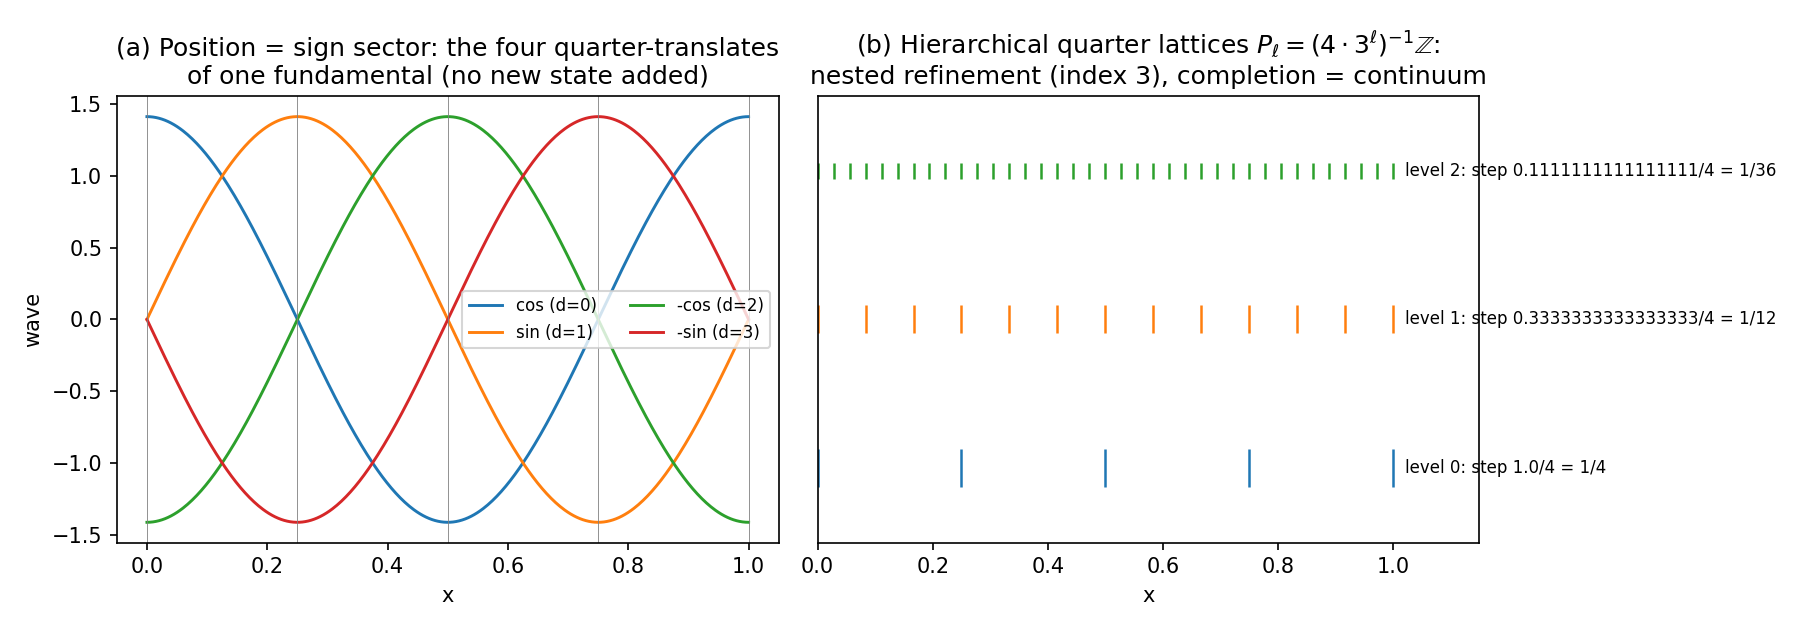
\includegraphics[width=1\linewidth,height=\textheight,keepaspectratio]{paper13_fig1_sign_sector.png}
- \textbf{図2}(\texttt{paper13\_fig2\_readout\_layers.png}):
読み出し三層の分離能 11⊂13⊂21(全2016対の全数計数)

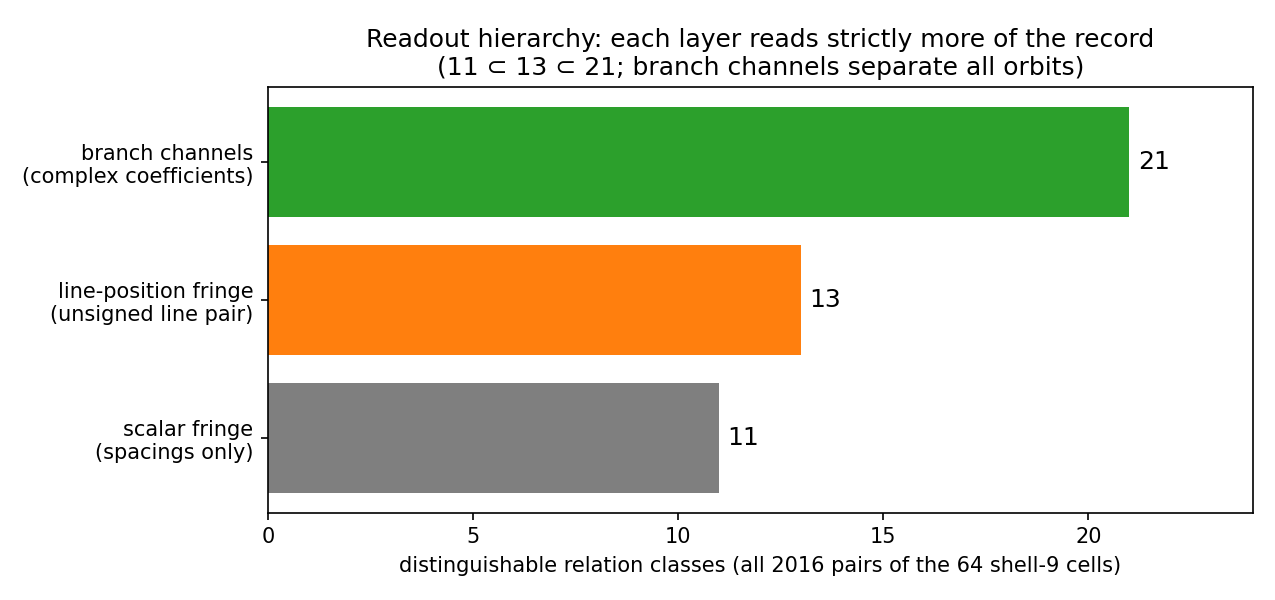
\includegraphics[width=1\linewidth,height=\textheight,keepaspectratio]{paper13_fig2_readout_layers.png}
- \textbf{図3}(\texttt{paper13\_fig3\_derived\_time.png}): (a)
時計標的=全奇数(199以下 100/100、間隔2)。(b) 刻み
\(\Delta t=1/\sqrt{s}\) --- t に独立の目盛りはない

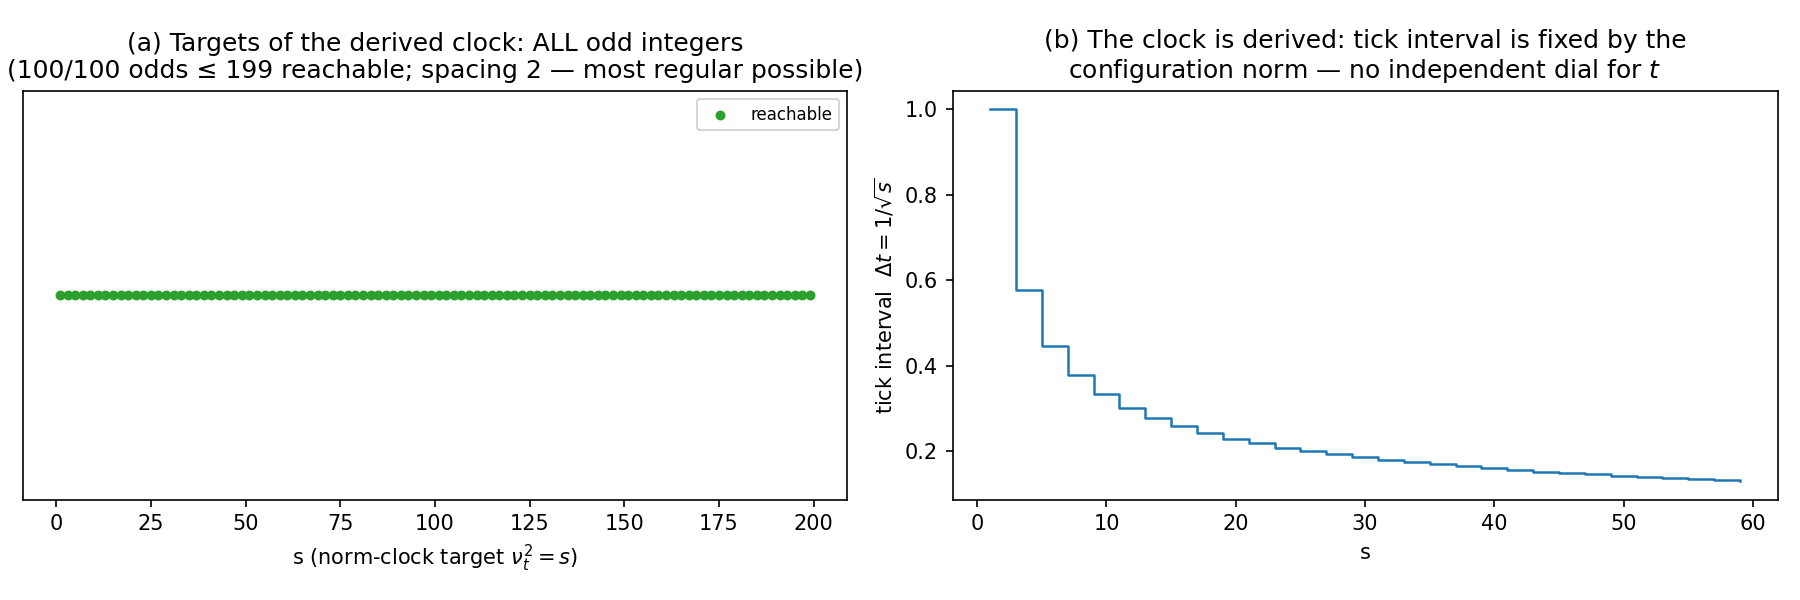
\includegraphics[width=1\linewidth,height=\textheight,keepaspectratio]{paper13_fig3_derived_time.png}

全図は実計算(模式図なし)。

\subsection{付録A:検証一覧(ラベル:①構成により真/②定理+機械確認/③落ちえた検査)}\label{ux4ed8ux9332aux691cux8a3cux4e00ux89a7ux30e9ux30d9ux30ebux2460ux69cbux6210ux306bux3088ux308aux771fux2461ux5b9aux7406ux6a5fux68b0ux78baux8a8dux2462ux843dux3061ux3048ux305fux691cux67fb}

{\def\LTcaptype{none} % do not increment counter
\begin{longtable}[]{@{}
  >{\raggedright\arraybackslash}p{(\linewidth - 8\tabcolsep) * \real{0.2000}}
  >{\raggedright\arraybackslash}p{(\linewidth - 8\tabcolsep) * \real{0.2000}}
  >{\raggedright\arraybackslash}p{(\linewidth - 8\tabcolsep) * \real{0.2000}}
  >{\raggedright\arraybackslash}p{(\linewidth - 8\tabcolsep) * \real{0.2000}}
  >{\raggedright\arraybackslash}p{(\linewidth - 8\tabcolsep) * \real{0.2000}}@{}}
\toprule\noalign{}
\begin{minipage}[b]{\linewidth}\raggedright
主張
\end{minipage} & \begin{minipage}[b]{\linewidth}\raggedright
ラベル
\end{minipage} & \begin{minipage}[b]{\linewidth}\raggedright
検証
\end{minipage} & \begin{minipage}[b]{\linewidth}\raggedright
方式
\end{minipage} & \begin{minipage}[b]{\linewidth}\raggedright
スクリプト
\end{minipage} \\
\midrule\noalign{}
\endhead
\bottomrule\noalign{}
\endlastfoot
定理1(¼並進=桁シフト) & ②(証明あり) & 4/4 & 全数確認 &
supplement62\_projection\_formalization.py \\
定理2a(双対性の一般論) & ---(証明事項・検証対象外) & --- & --- & --- \\
定理2b(Z₄↪U(1) 整合) & ② & 定理1 と同一の 4/4 & 全数確認 & 同上 \\
定理3(11/13/21) & ③ & 全2016対 & \textbf{全数} &
supplement79\_scale\_free\_and\_stripe\_table.py・supplement81\_mirror\_lemma\_check.py(スカラー縞)・paper13\_14\_figures.py \\
21軌道の完全分離(枝チャネル) & ③ & 21/21 & 全数 &
supplement44\_branch\_channel\_verification.py \\
定理4(変位の可読性) & ③ & 縞シフトテスト2件 PASS & \textbf{標本} &
supplement44\_branch\_channel\_verification.py \\
定理5(全奇数) & ②(ガウスの定理による証明あり) & 奇数≤199 100/100 &
範囲内確認 & paper13\_14\_figures.py \\
定理6(t 因子化) & ②(在庫監査スケッチ) & 論文15 往復 500/500 が実現の確認
& 照合 & supplement62\_inverse\_roundtrip\_test.py \\
\end{longtable}
}

\begin{center}\rule{0.5\linewidth}{0.5pt}\end{center}

\textbf{謝辞・履歴}: 検証は Claude Code(ローカル機械検証)と
claude.ai(独立検算)の二者独立検算プロトコルによる。検算範囲の正確な記載:64セル域の三層計数(11/13/21)は
Claude Code 検証+claude.ai は48セル域(13/8)で方法同値確認まで ---
64域の独立再計算は claude.ai 側のキューに登録済み。定理5
の証明はガウスの三角数定理の同定(claude.ai、第1回査読 \#1)による。定理6
の原型は補遺48(2026-06-12)による。素材:補遺43・44・47(枝チャネル部分のみ)・48・79・81(2026-06-12)。v0.2:第1回査読(中改訂)\#1〜\#14
反映。v1.0:第2回査読(採録・軽微条件付き)R1〜R5 反映。

物理的同一視は行わない。

\end{document}
